\documentclass{article}

\usepackage{fancyhdr}
\usepackage{extramarks}
\usepackage{amsmath}
\usepackage{amsthm}
\usepackage{amsfonts}
\usepackage{tikz}
\usepackage[plain]{algorithm}
\usepackage{algpseudocode}

\usetikzlibrary{automata,positioning}

%
% Basic Document Settings
%

\topmargin=-0.45in
\evensidemargin=0in
\oddsidemargin=0in
\textwidth=6.5in
\textheight=9.0in
\headsep=0.25in

\linespread{1.1}

\pagestyle{fancy}
\rhead{\firstxmark}
\lfoot{\lastxmark}
\cfoot{\thepage}

\renewcommand\headrulewidth{0.4pt}
\renewcommand\footrulewidth{0.4pt}

\setlength\parindent{0pt}

%
% Create Problem Sections
%

\newcommand{\enterProblemHeader}[1]{
    \nobreak\extramarks{}{Problem \arabic{#1} continued on next page\ldots}\nobreak{}
    \nobreak\extramarks{Problem \arabic{#1} (continued)}{Problem \arabic{#1} continued on next page\ldots}\nobreak{}
}

\newcommand{\exitProblemHeader}[1]{
    \nobreak\extramarks{Problem \arabic{#1} (continued)}{Problem \arabic{#1} continued on next page\ldots}\nobreak{}
    \stepcounter{#1}
    \nobreak\extramarks{Problem \arabic{#1}}{}\nobreak{}
}

\setcounter{secnumdepth}{0}
\newcounter{partCounter}
\newcounter{homeworkProblemCounter}
\setcounter{homeworkProblemCounter}{1}
\nobreak\extramarks{Problem \arabic{homeworkProblemCounter}}{}\nobreak{}

%
% Homework Problem Environment
%
% This environment takes an optional argument. When given, it will adjust the
% problem counter. This is useful for when the problems given for your
% assignment aren't sequential. See the last 3 problems of this template for an
% example.
%
\newenvironment{homeworkProblem}[1][-1]{
    \ifnum#1>0
        \setcounter{homeworkProblemCounter}{#1}
    \fi
    \section{Problem \arabic{homeworkProblemCounter}}
    \setcounter{partCounter}{1}
    \enterProblemHeader{homeworkProblemCounter}
}{
    \exitProblemHeader{homeworkProblemCounter}
}



%
% Homework Details
%   - Title
%   - Due date
%   - Class
%   - Section/Time
%   - Instructor
%   - Author
%

\newcommand{\hmwkTitle}{Homework\ \#3 Part 1}
\newcommand{\hmwkName}{Probabilistic Reasoning}
\newcommand{\hmwkDate}{April 14, 2023}
\newcommand{\hmwkClass}{CS 440: Introduction to Artificial Intelligence}
\newcommand{\hmwkClassInstructor}{Professor Abdelsam Boularias}


%
% Title Page
%

\title{
    \vspace{2in}
    \textmd{\textbf{\hmwkClass}}\\
    \textmd{\hmwkTitle\ \hmwkName}\\
    \vspace{0.1in}\small{\hmwkDate}\\
    \vspace{0.1in}\large{\textit{\hmwkClassInstructor}}
    \vspace{3in}
}

\author{
    \textbf{Jay Patwardhan} {208001851}\\ 
    \textbf{Alan Wu} {208000574}\\ 
    \textbf{Neel Shejwalkar} {207004853}
}
\date{}

\renewcommand{\part}[1]{\textbf{\large Part \Alph{partCounter}}\stepcounter{partCounter}\\}

%
% Various Helper Commands
%

% Useful for algorithms
\newcommand{\alg}[1]{\textsc{\bfseries \footnotesize #1}}

% For derivatives
\newcommand{\deriv}[1]{\frac{\mathrm{d}}{\mathrm{d}x} (#1)}

% For partial derivatives
\newcommand{\pderiv}[2]{\frac{\partial}{\partial #1} (#2)}

% Integral dx
\newcommand{\dx}{\mathrm{d}x}

% Alias for the Solution section header
\newcommand{\bruh}{\textbf{\large Solution}}
\newtheorem*{solution*}{Solution}
\newenvironment{solution}{\begin{solution*}}{{\finishline} \end{solution*}}


% Probability commands: Expectation, Variance, Covariance, Bias
\newcommand{\E}{\mathrm{E}}
\newcommand{\Var}{\mathrm{Var}}
\newcommand{\Cov}{\mathrm{Cov}}
\newcommand{\Bias}{\mathrm{Bias}}

\begin{document}

\maketitle

\pagebreak

%Part 1%
\begin{homeworkProblem}
    \textbf{\large Consider the following Bayesian network, where variables A through E are all Boolean valued. Note: there is a typo in the image, it should be $P(A = true) = 0.2$ instead of $P(D = true) = 0.2$}\\\\
    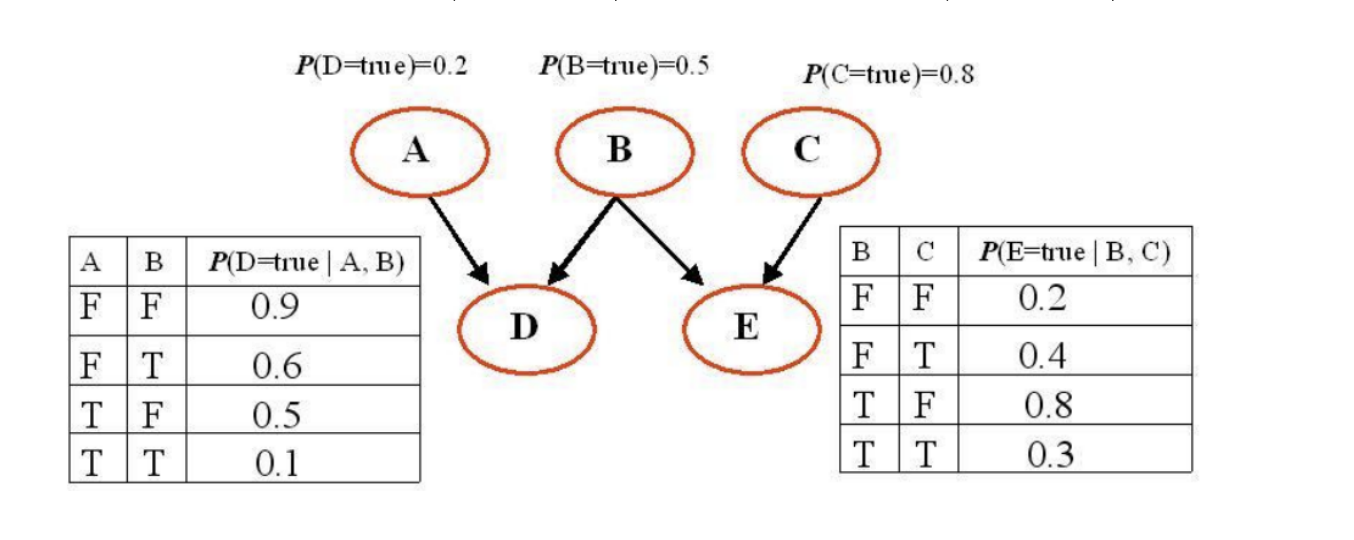
\includegraphics[width=1\textwidth]{Problem1.png}

    \part 
    
    \textbf{What is the probability that all five of these Boolean variables are simultaneously true? [Hint: You have to compute the joint probability distribution. The structure of the Bayesian network suggests how
    the joint probability distribution is decomposed to the conditional probabilities available]}\\
    $P(A,B,C,D,E) = P(A) \cdot P(B) \cdot P(C) \cdot P(D | A=T, B=T) \cdot P(E | B=T, C=T) \\
 = 0.2 \cdot 0.5 \cdot 0.8 \cdot 0.1 \cdot 0.3 = 0.0024$\\

    \part 
    
    \textbf{What is the probability that all five of these Boolean variables are simultaneously false? [Hint: Answer similarly to above.]}\\
     $P(\neg A,\neg B, \neg C, \neg D, \neg E) = P(\neg A) = P(\neg A) \cdot P(\neg B) \cdot P(\neg C) \cdot P(\neg D | A=F, B=F) \cdot P(\neg E | B=F, C=F) \\
     = (1-0.2) \cdot (1-0.5) \cdot (1-0.8) \cdot (1-0.9) \cdot (1-0.2) \\
     = 0.8 \cdot 0.5 \cdot 0.2 \cdot 0.1 \cdot 0.8 = 0.0064$\\

    \part 
    
    \textbf{What is the probability that A is false given that the four other variables are all known to be true?}\\
    $P(\neg A | B, C, D, E) = \frac{P(\neg A, B, C, D, E)}{P(B,C,D,E)}$\\
    $P(\neg A, B, C, D, E) = P(\neg A) \cdot P(B) \cdot P(C) \cdot P(D | A=F, B=T) \cdot P(E | B=T, C=T) \\
    = (1-0.2) \cdot 0.5 \cdot 0.8 \cdot 0.6 \cdot 0.3 = 0.0576$\\
    $P(B,C,D,E) = P(A,B,C,D,E) + P(\neg A, B, C, D, E) = 0.0024 + 0.0576 = 0.06$\\
    $P(\neg A | B, C, D, E) = \frac{0.0576}{0.06} = 0.96$


\end{homeworkProblem}

\pagebreak

%Part 2%
\begin{homeworkProblem}
    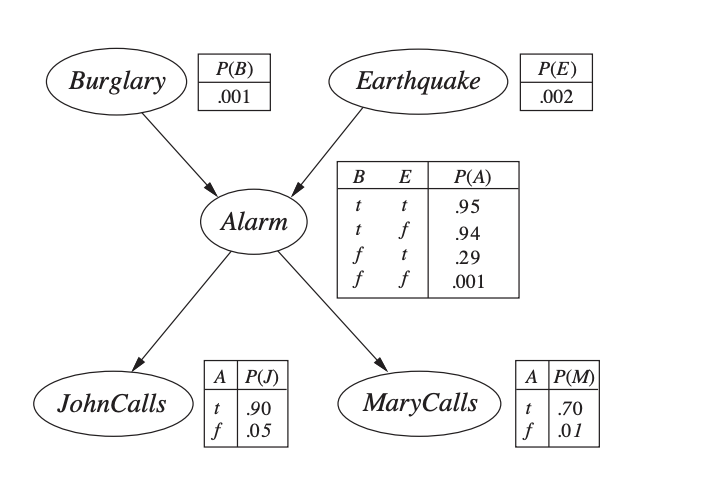
\includegraphics[width=1\textwidth]{Problem2.png}

    \part 
    \textbf{Calculate $P(Burglary | JohnsCalls = true, MaryCalls = true)$ and show in detail the calculations that take place. Use your book to confirm that your answer is correct.}\\

    The enumeration tree is shown:\\

    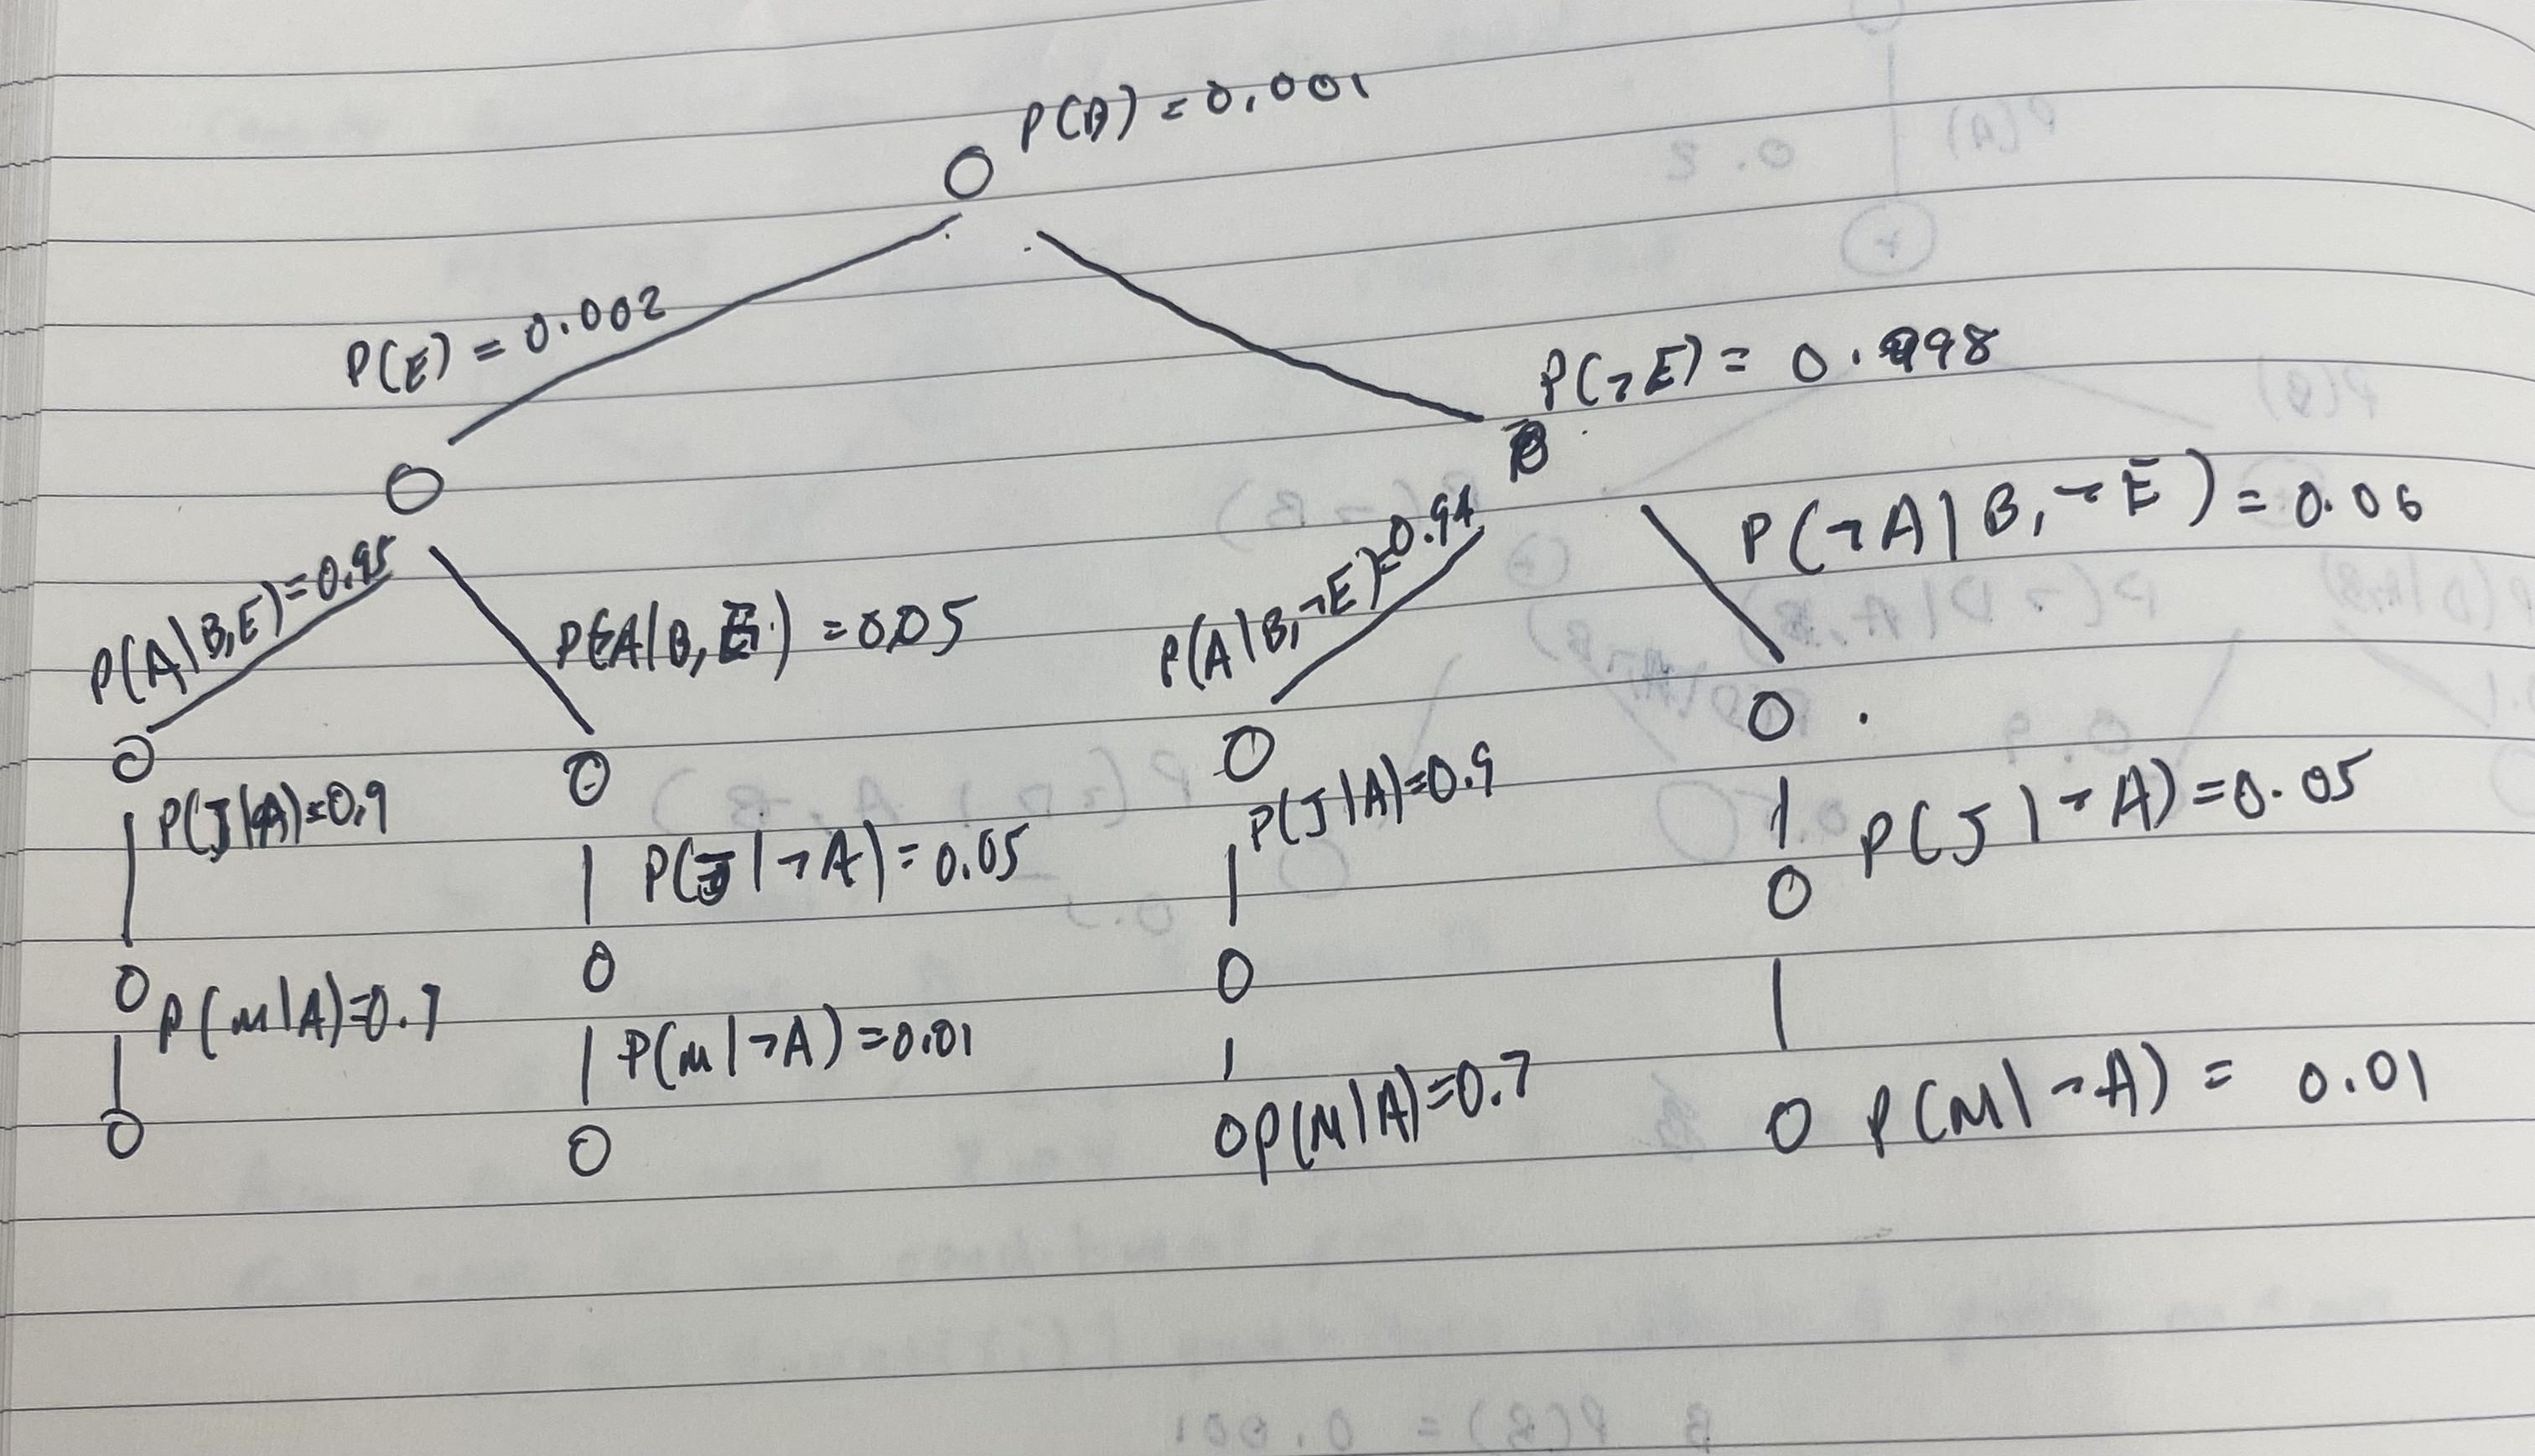
\includegraphics[width=1\textwidth]{BurglarEnumerate.jpg}


    $P(Burglary | JohnsCalls = true, MaryCalls = true) = P(B) \cdot \frac{P(J,M | B)}{P(J,M)}\\
    = 0.001 \cdot \frac{(P(A|B) \cdot P (J,M|A)) + (P(\neg A|B) \cdot P(J,M|\neg A)) }{(P(J,M|A) \cdot P(A)) +(P(J,M|\neg A) \cdot P(\neg A))}$\\

    $P(A|B) = \frac{P(A \cap B)}{P(B)} = \frac{(P(B) \cdot P(E) \cdot P(A|B,E))+(P(B) \cdot P(\neg E) \cdot P(A|B, \neg E))}{P(B)}\\
    = \frac{(0.001 \cdot 0.002 \cdot 0.95)+(0.001 \cdot 0.998 \cdot 0.94)}{0.001} = 0.94002$\\

    $P(J,M|A) = P(J|A) \cdot P(M|A) = 0.9 \cdot 0.7 = 0.63$\\

    $P(J,M|\neg A) = P(J|\neg A) \cdot P(M|\neg A) = 0.05 \cdot 0.01 = 0.0005$\\

    $P(\neg A|B) = 1-P(A|B) = 1-0.94002 = 0.05998$\\

    $P(A) = (P(B)\cdot P(E) P(A|B,E)) + (P(B) \cdot P(\neg E) P(A|B,\neg E)) + (P(\neg B) \cdot P(E) \cdot P(A|\neg B, E)) + (P(\neg B) \cdot P(\neg E) \cdot P(A|\neg B, \neg E)) \\
    = (0.001 \cdot 0.002 \cdot 0.95) + (0.001 \cdot 0.998 \cdot 0.94) + (0.999 \cdot 0.002 \cdot 0.29) + (0.999 \cdot 0.998 \cdot 0.001)\\
    = 0.0025$\\

    $P(\neg A) = 1-P(A) = 1-0.0025 = 0.99748$\\

    Therefore: 

    $P(Burglary | JohnCalls = true, MaryCalls = true) = 0.001 \cdot \frac{(0.94002 \cdot 0.63) + (0.05998 \cdot 0.0005)}{(0.63 \cdot 0.0025)+(0.0005 \cdot 0.99748)}\\
    = 0.2841718$\\



    

    \part
    \textbf{Suppose a Bayesian network has the from of a $chain:$ a sequence of Boolean variables $X_1,....X_n$ where $Parents(X_i) = X_{i-1}$ for $i = 2, ...., n$. What is the complexity of computing $P(X_1|Xn = true)$ using enumeration. What is the complexity with variable elimination?}\\

    The complexity for Enumeration: \\
    
    Above is the binary tree since we only care about the true values for $X_1$ and $X_N$. We are looking for $P(X_1|X_n = true)$. Given the tree above, we know that the binary tree will have $n$ levels that branch $n-2$ times. With the graph shown with 5 levels, it only branches 3 times. The above graph is missing the top level node. In this tree design there is a total of $2^{n-1}$ nodes. The space complexity will be $O(n)$ for dfs to traverse the tree and it will take $O(2^{n})$ time complexity, with $2^{n-1}$ nodes absorbed into $2^n$. \\

    Now we will calculate the complexity for variable elimination: \\

    $P(X_1 | X_n = True) \\
    = \alpha P(X_1) \sum_{X_2}{P(X_2|X_1)}\sum_{X_3}{P(X_3|X_2)}...\cdot \sum_{X_{n-2}}{X_{n-2}|X_{n-3}}\sum_{X_{n-1}}{X_{n-1}|X_{n-2}}\cdot P(X_n|X_{n-01}) \\
    = \alpha \sum_{X_2} \sum_{X_3} ... \sum_{X_{n-1}}{f_1(X_1)xf_2(X_2)xf_{n-1}(X_{n-1})xf_n(X_n)}$\\

    Each $f_k(X_k)$ term is a $2x1$ matrix that has $X_K | X_{K-1}$ on the top and $\neg X_K | X_{K-1}$ on the bottom. The total space complexity is $2n$ and therefore $O(n)$. The total time complexity is the time to multiply all the matrices, which is $2n$. This absorbs to runtime time complexity of $O(n)$





\end{homeworkProblem}

\pagebreak

%Part 3%
\begin{homeworkProblem}
    \textbf{\large Suppose you are working for a financial institution and you are asked to implement a fraud detection system. You plan to use the following information: }

    \begin{itemize}
        \item When the card holder is travelling abroad, fraudulent transactions are more likely since tourists are prime targets for
        thieves. More precisely, 1\% of transactions are fraudulent when the card holder is travelling, where as only 0.4\%
        of the transactions are fraudulent when she is not travelling. On average, 5\% of all transactions happen while the
        card holder is travelling. If a transaction is fraudulent, then the likelihood of a foreign purchase increases, unless the
        card holder happens to be travelling. More precisely, when the card holder is not travelling, 10\% of the fraudulent
        transactions are foreign purchases where as only 1\% of the legitimate transactions are foreign purchases. On the
        other hand, when the card holder is travelling, then 90\% of the transactions are foreign purchases regardless of the
        legitimacy of the transactions.
        \item Purchases made over the internet are more likely to be fraudulent. This is especially true for card holders who don’t
        own any computer. Currently, 75\% of the population owns a computer or smart phone and for those card holders,
        1\% of their legitimate transactions are done over the internet, however this percentage increases to 2\% for fraudulent
        transactions. For those who don’t own any computer or smart phone, a mere 0.1\% of their legitimate transactions
        is done over the internet, but that number increases to 1.1\% for fraudulent transactions. Unfortunately, the credit
        card company doesn’t know whether a card holder owns a computer or smart phone, however it can usually guess by
        verifying whether any of the recent transactions involve the purchase of computer related accessories. In any given
        week, 10\% of those who own a computer or smart phone purchase (with their credit card) at least one computer
        related item as opposed to just 0.1\% of those who don’t own any computer or smart phone.
    \end{itemize}
    \part

    \textbf{Construct a Bayes Network to identify fraudulent transactions.}

    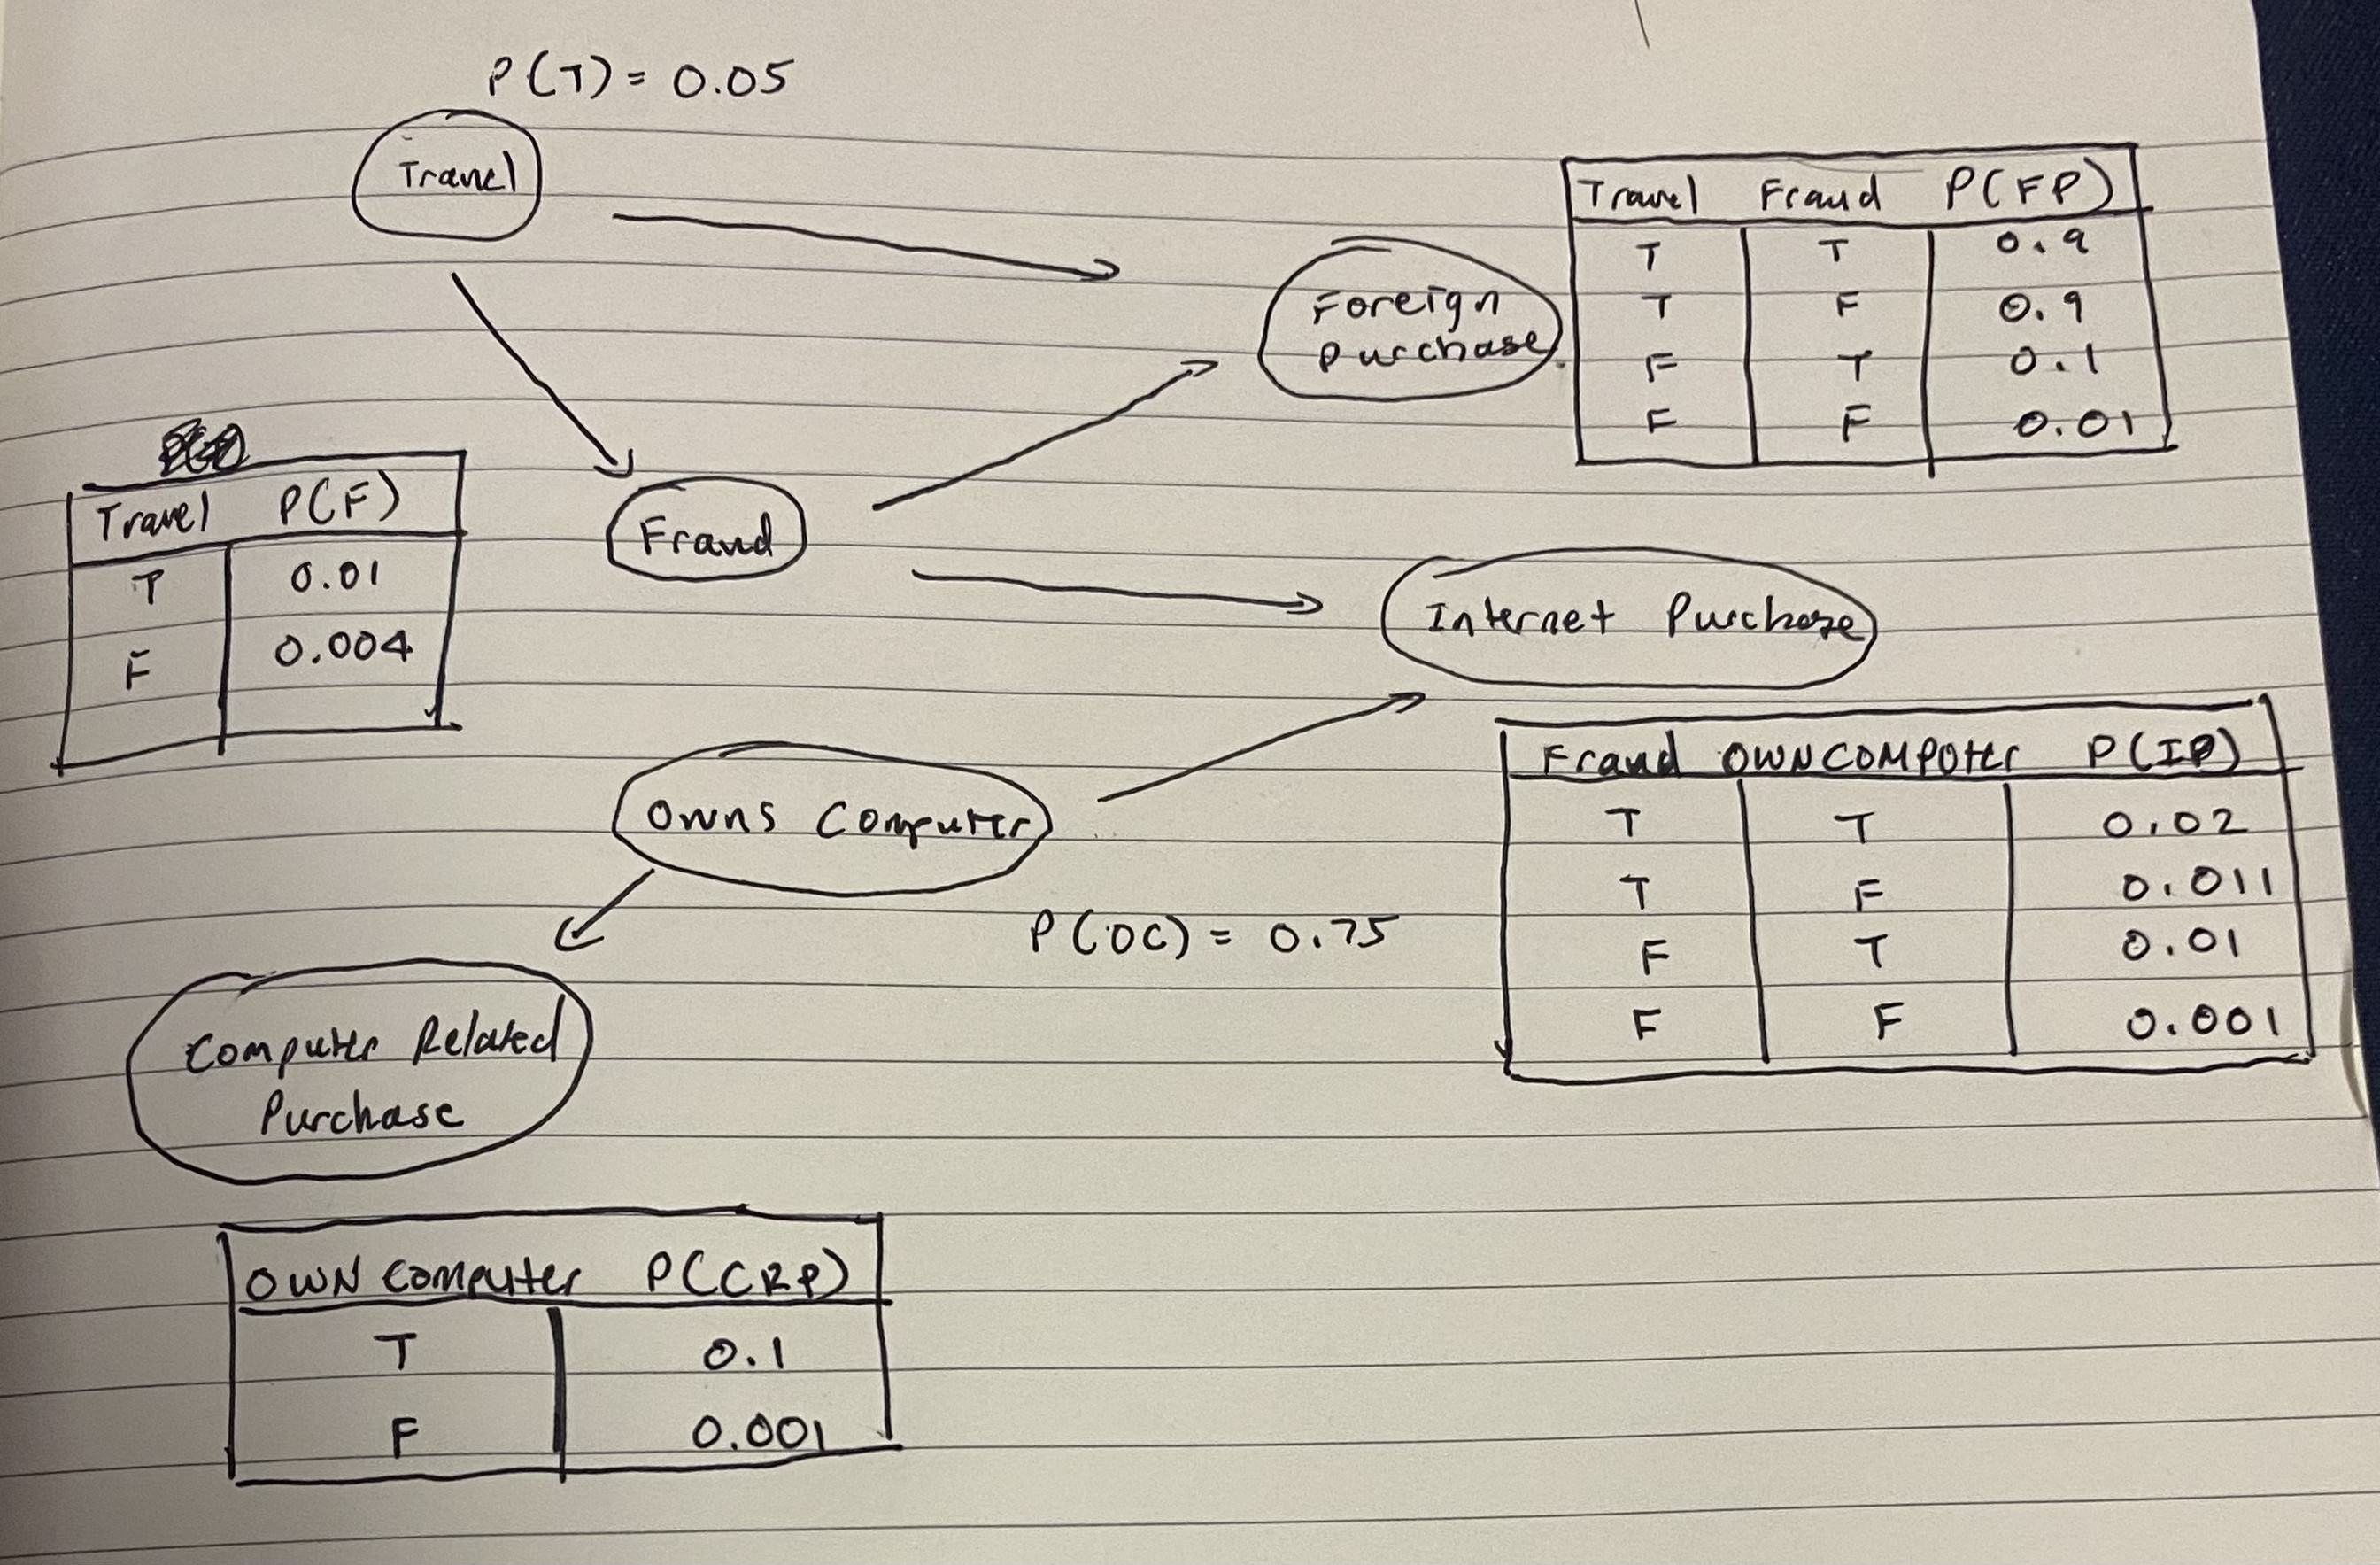
\includegraphics[width=1\textwidth]{P3Network.jpg}

    \part

    \textbf{What is the prior probability (i.e., before we search for previous computer related purchases and before we verify
    whether it is a foreign and/or an internet purchase) that the current transaction is a fraud? What is the probability that
    the current transaction is a fraud once we have verified that it is a foreign transaction, but not an internet purchase
    and that the card holder purchased computer related accessories in the past week?}

    The probabilities we want to search for: $P(Fraud)$ and $P(Fraud | FP=T, IP=F, CRP=T)$.\\

    Part 1: $P(Fraud)$\\
    $P(Fraud) \\
    = (P(F|Trav) \cdot P(Trav)) + (P(F|\neg Trav) \cdot P(\neg Trav))\\
    = (0.01 \cdot 0.05) + (0.004 \cdot 0.95) = 0.0043$\\

    Part 2: \\
        ${P(Fraud | FP, \neg IP, CRP)} \\
        = \frac{1}{\alpha} \cdot \sum_{Trav,OC}{P(Fraud | FP, \neg IP, CRP)} \\
        = \frac{1}{\alpha} \cdot \sum_{Trav,OC}{P(Trav) \cdot P(Fraud|Trav) \cdot P(FP|Fraud,Trav) \cdot P(OC) \cdot P(CRP,OC) \cdot P(\neg IP|OC,Fraud) } \\
        $\\

        All cases: 
        \begin{enumerate}
            \item $Trav = True, OC = True$\\
            Total Probability = $0.05 \cdot 0.01 \cdot 0.9 \cdot 0.75 \cdot 0.1 \cdot (1-0.02) = 0.000033075$
            \item $Trav = True, OC = False$\\
            Total Probability = $0.05 \cdot 0.01 \cdot 0.9 \cdot 0.25 \cdot 0.001 \cdot (1-0.011) = 0.0000001112625$
            \item $Trav = False, OC = True$\\
            Total Probability = $0.95 \cdot 0.004 \cdot 0.1 \cdot 0.75 \cdot 0.1 \cdot (1-0.02) = 0.00002793$
            \item $Trav = False, OC = False$\\
            Total Probability = $0.95 \cdot 0.004 \cdot 0.1 \cdot 0.25 \cdot 0.001 \cdot (1-0.011) = 0.000000093955$
        \end{enumerate}
        
        $P(Fraud | FP, \neg IP, CRP) \\
        = \frac{1}{\alpha} \cdot 0.000033075 + 0.0000001112625 + 0.00002793 + 0.000000093955 \\
        = \frac{1}{\alpha} \cdot 0.00006121021\\
        = \frac{1}{0.00006121021 + 0.01026} \cdot 0.00006121021 = 0.00592$
   
\end{homeworkProblem}
\end{document}